\documentclass[main.tex]{subfiles}
%% Current Author:
\setcounter{chapter}{13}
\begin{document}
\chapter{Electromagnetism}
\spec{understand and use the terms magnetic flux density, flux and flux linkage}

Electromagnetic induction depends crucially on the concept of \emph{flux}. This is the product of the magnetic field strength $B$ and the area of a loop perpendicular to the field, $A$.
\[ \Phi = BA \]
The unit of flux is the weber, Wb. Given its relation to flux, the field strength $B$ can also be referred to as the magnetic flux density. It also follows that the tesla is equivalent to one weber per metre-squared.

When a coil of wire encloses an area of flux we can calculate the \emph{flux-linkage} which is the product of the flux through the coil and the number of turns on the coil, $N\Phi$.

\spec{understand that magnetic fields are created by electric current}

An electric current in a wire creates a magnetic field. The field strength depends on the size of the current and the distance from the wire. In the case of a solenoid or electromagnet the field strength is also proportional to the number of turns on the coil.

\spec{recognise and use  $F = BIl\sin\theta$}

This is the equation for the force on a current-carrying wire of length $l$ with a current of $I$ at an angle $\theta$ to a magnetic field of strength $B$.

\spec{recognise and use $F = BQv\sin\theta$}

This is the equation for a particle of charge $Q$ moving at a velocity $v$ at an angle $\theta$ to a magnetic field of strength $B$.

\spec{use Fleming's left-hand rule to solve problems}

Fleming's left-hand rule allows the calculation of the direction of the force on either a charged particle or a current-carrying wire. The geometry is shown below.

\begin{figure}[h]
  \begin{center}
  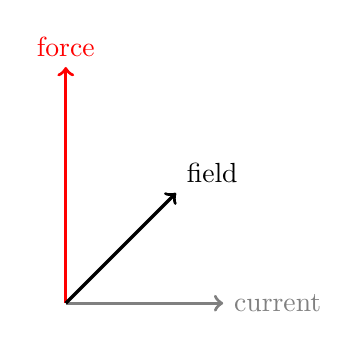
\begin{tikzpicture}
      \draw [->, gray,very thick] (0,0) -- (2,0) node[anchor=west] {current};
      \draw [->, red,very thick] (0,0) -- (0,3) node[anchor=south] {force};
      \draw [->, black,very thick] (0,0) -- (1.4,1.4) node[anchor=south west] {field};
    \end{tikzpicture}
  \end{center}
  \caption{Fleming's left-hand rule}
  \label{flemminglh}
\end{figure}

\spec{explain qualitatively the factors affecting the emf induced across a coil when there is relative motion between the coil and a permanent magnet or when there is a change of current in a primary coil linked with it}
\spec{recognise and use $E=-\frac{d(N\Phi)}{dt}$ and explain how it is an expression of Faraday’s and Lenz’s laws}
\spec{derive, recall and use $r = \frac{mv}{BQ}$ for the radius of curvature of a deflected charged particle}
\spec{explain the Hall effect, and derive and use $V = Bvd$}
\end{document}
